% !TEX output_directory = ./build

%%%%%%%%%%%%%%%%%%%%%%%%%%%%%%%%%%%%%%%%%%%%%%%%%%%%%%%%%%%%%%%%%%%%%%%%
% Autonomous Intelligent System, University of Bonn, LaTeX Beamer theme
%
% Copyright (C) 2010-2013 Dirk Holz, dirk.holz@ieee.org

% This program is free software: you can redistribute it and/or modify
% it under the terms of the GNU General Public License as published by
% the Free Software Foundation, either version 3 of the License, or
% (at your option) any later version.

% This program is distributed in the hope that it will be useful,
% but WITHOUT ANY WARRANTY; without even the implied warranty of
% MERCHANTABILITY or FITNESS FOR A PARTICULAR PURPOSE.  See the
% GNU General Public License for more details.

% You should have received a copy of the GNU General Public License
% along with this program.  If not, see <http://www.gnu.org/licenses/>.

\documentclass[pdftex, handout]{beamer}
\let\Tiny=\tiny

% all available options --->
% \usetheme[shadow,logoinnavbar,subsection,logoinframe,framenavbar]{AIS}
\usetheme[shadow,logoinnavbar,subsection]{AIS}

\usepackage{listings}
\usepackage{array} % needed for \arraybackslash
\usepackage{graphicx}
\usepackage{adjustbox} % for \adjincludegraphics
\usepackage{tikz}
\usetikzlibrary{shapes.geometric,shapes.arrows,decorations.pathmorphing}
\usetikzlibrary{matrix,chains,scopes,positioning,arrows,fit}
% \scalebox{<h-scale>}[<v-scale>]{<content>}


\title[Solving localization problem in first person computer games with deep learning]{Master seminar: Solving localization problem in first person computer games with deep learning}
% \subtitle{}
\author[Y.Selivonchyk]{\highlight{  Yauheni Selivonchyk}\inst{1}, \\
Prof. Dr. Christian Bauckhage\inst{2}, \\
Prof. Dr. Stefan Wrobel\inst{2}, \\
  Mr. Sc. Rafet Sifa\inst{2} \\
}
\institute[University of Bonn]
{
  \inst{1}%
  Institute of Computer Science, University of Bonn
  \and
  \inst{2}Fraunhofer IAIS
}

\date{\today}

% This is only inserted into the PDF information catalog. Can be left out.
\subject{Talks}

% Delete this, if you do not want the table of contents to pop up at
% the beginning of each subsection:
% \AtBeginSection[]
% {
%   \begin{frame}<beamer>
%     \frametitle{Outline}
%     \tableofcontents[currentsection]
%   \end{frame}
% }

% If you wish to uncover everything in a step-wise fashion, uncomment
% the following command:
% \beamerdefaultoverlayspecification{<+->}

\begin{document}

\begin{frame}
  \titlepage
\end{frame}

\begin{frame}
  \frametitle{Outline}
  \tableofcontents
  % \tableofcontents[pausesections]
\end{frame}


\section{Introduction}

\subsection{Unsupervised learning}

\begin{frame}{Importance of unsupervised learning for AI}
   \begin{figure}
   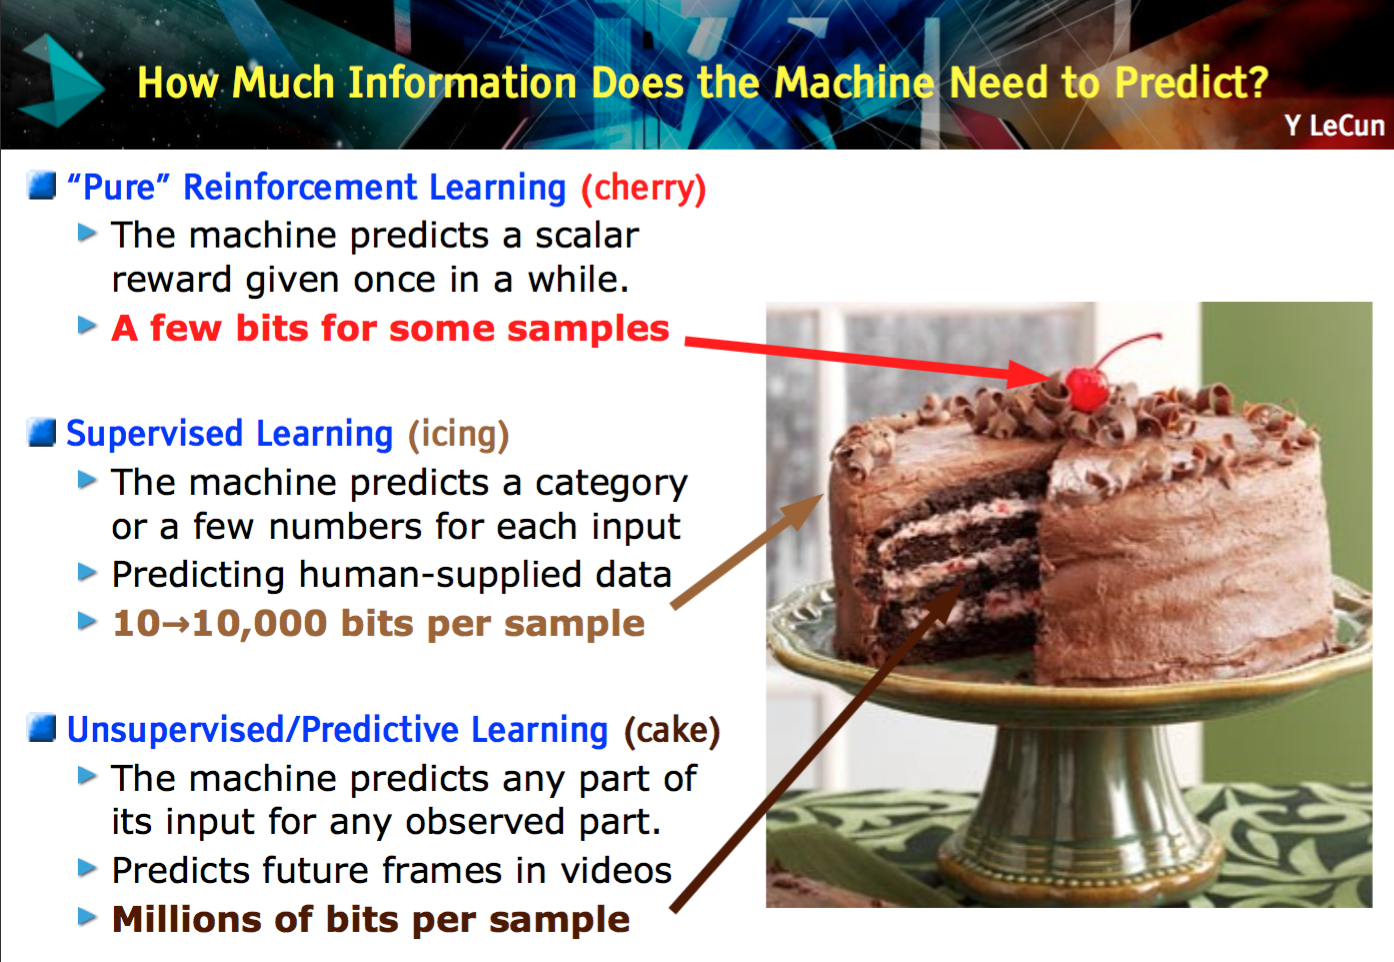
\includegraphics[width=0.8\textwidth,height=0.8\textheight,keepaspectratio]{images/lecun_nips.png}
 \caption{Slide from "Predictive learning" opening address given by Yann Lecun at NIPS2016.}
 \end{figure}
\end{frame}

\begin{frame}{Key components of finding a solutions}
  \begin{itemize}
    \item Sufficient amount of training data
  \end{itemize}
  \begin{itemize}
    \item Computational feasibility of the problem
  \end{itemize}
\end{frame}


\subsection{Localization problem}

\begin{frame}{Localization}
  Localization as a task of extracting, tracking or predicting object's position in some environment from available sensory data
\end{frame}

\begin{frame}{Localization example: Tracking}
  \begin{figure}
  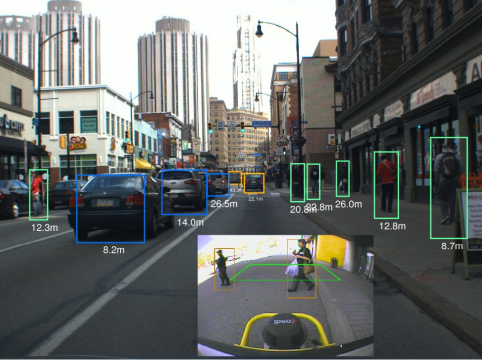
\includegraphics[width=0.5\textwidth,height=0.5\textheight,keepaspectratio]{images/tracking.png}
\caption{Pedestrian tracking visualization \footnotemark.}
\end{figure}
\footnotetext[1]{H. Cho et. al. "Real-Time Pedestrian and Vehicle Detection for Automotive Active Safety Systems"}

\end{frame}

\begin{frame}[noframenumbering]{Localization example: SLAM}
  \begin{figure}
  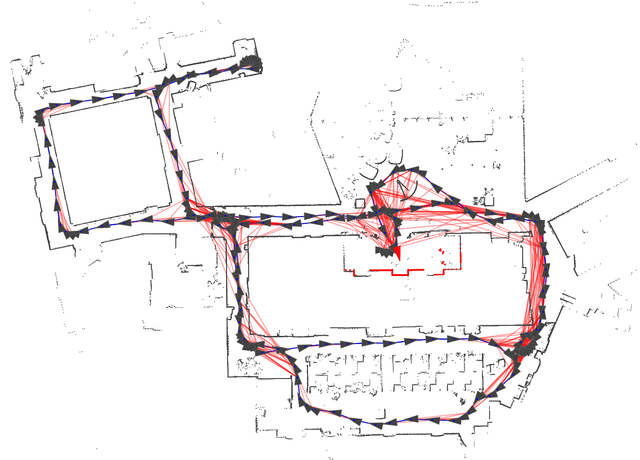
\includegraphics[width=0.8\textwidth,height=0.7\textheight,keepaspectratio]{images/slam.png}
\caption{Example solution of SLAM problem on PC3 dataset (courtesy of University of Michigan).}
\end{figure}
\end{frame}

\begin{frame}[noframenumbering]{Localization example: surgery}
  \begin{figure}
  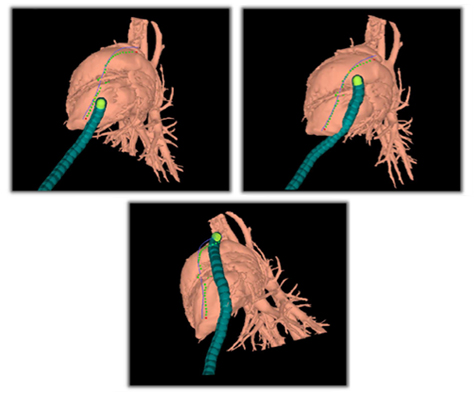
\includegraphics[width=0.8\textwidth,height=0.7\textheight,keepaspectratio]{images/slam_surg.jpg}
\caption{Mapping the position of a tool in minimally invasive surgery [http://biorobotics.ri.cmu.edu/research/medicalSLAM.html].}
\end{figure}

\end{frame}

\begin{frame}{Motivation. Continuied}
  Goal of this work: reconstruction of the actors trajectory in first-person shooter (games) from visual data.

  \pause

  \begin{figure}
    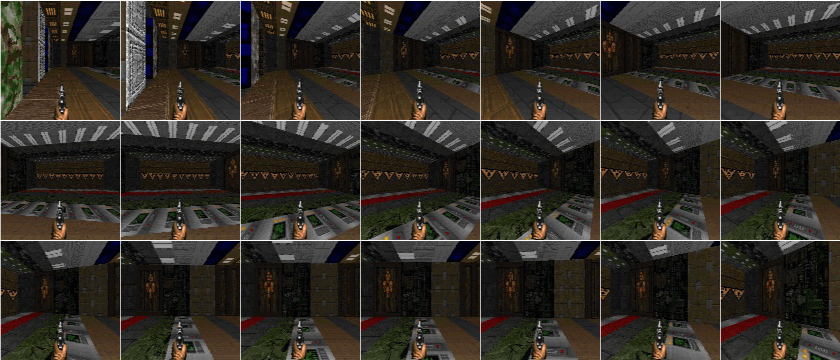
\includegraphics[width=0.8\textwidth,height=0.7\textheight,keepaspectratio]{images_main/sprite2.png}
  \caption{Example visual data.}
  \end{figure}
\end{frame}


\section{Approach}

% \subsection{Spatial embedding model}
%
% \begin{frame}
%   \begin{tabular}{p{.3\textwidth} p{.7\textwidth}}
%   \adjincludegraphics[width=.8\linewidth,valign=t]{images/slam.png}
%   &
%   \raggedright\arraybackslash\textbf{The problem of distinguishing prime numbers from composites, and of resolving composite numbers into their prime factors, is one of the most important and useful in all of arithmetic.}
%
%   \hfill-- Carl Friedrich Gauss
%   \end{tabular}
%
% \end{frame}

\subsection{Model design}

\begin{frame}{Autoencoder model}
  \textbf{Autoencoders} learn to project the input $x$ into some embedding space $h \in H$ and simultaneously reconstruct the original information $\hat{x}$.
  \pause
\vspace{1cm}

    \begin{tabular}{p{.5\textwidth} p{.5\textwidth}}
    \adjincludegraphics[width=.9\linewidth,valign=t]{images/ae2.png}
    &
    \begin{itemize}
      \item $f: \Bbb{R}^N \to \Bbb{R}^M$
      \item $g: \Bbb{R}^M \to \Bbb{R}^N$
    \end{itemize}
    \end{tabular}
\end{frame}

\begin{frame}{Model pre-training. Motivation}
  Extremely high compression rates 76200 (160*120*4) $\to$ 3..6 are notoriously difficult to learn.
\end{frame}


\begin{frame}{Common irregularities in the manifold space}
  \begin{enumerate}
  \item High density region \\
  \item Low density regions \\
  \item High curvature of the manifold \\
  \end{enumerate}
\end{frame}


\begin{frame}[noframenumbering]{Common irregularities in the manifold space}
  \begin{enumerate}
  \item High density region \\
    - Apply random noise in the encoding space to increase "save" distance between frames
  \item Low density regions \\
    - Add "max-distance" penalty
  \item High curvature of the manifold \\
    - Regularize local continuity of in the embedding space
  \end{enumerate}
\end{frame}


\begin{frame}{Predictive regularization}
  Try to estimate positional encoding of the next frame using last two frames of the video.
  \begin{figure}
    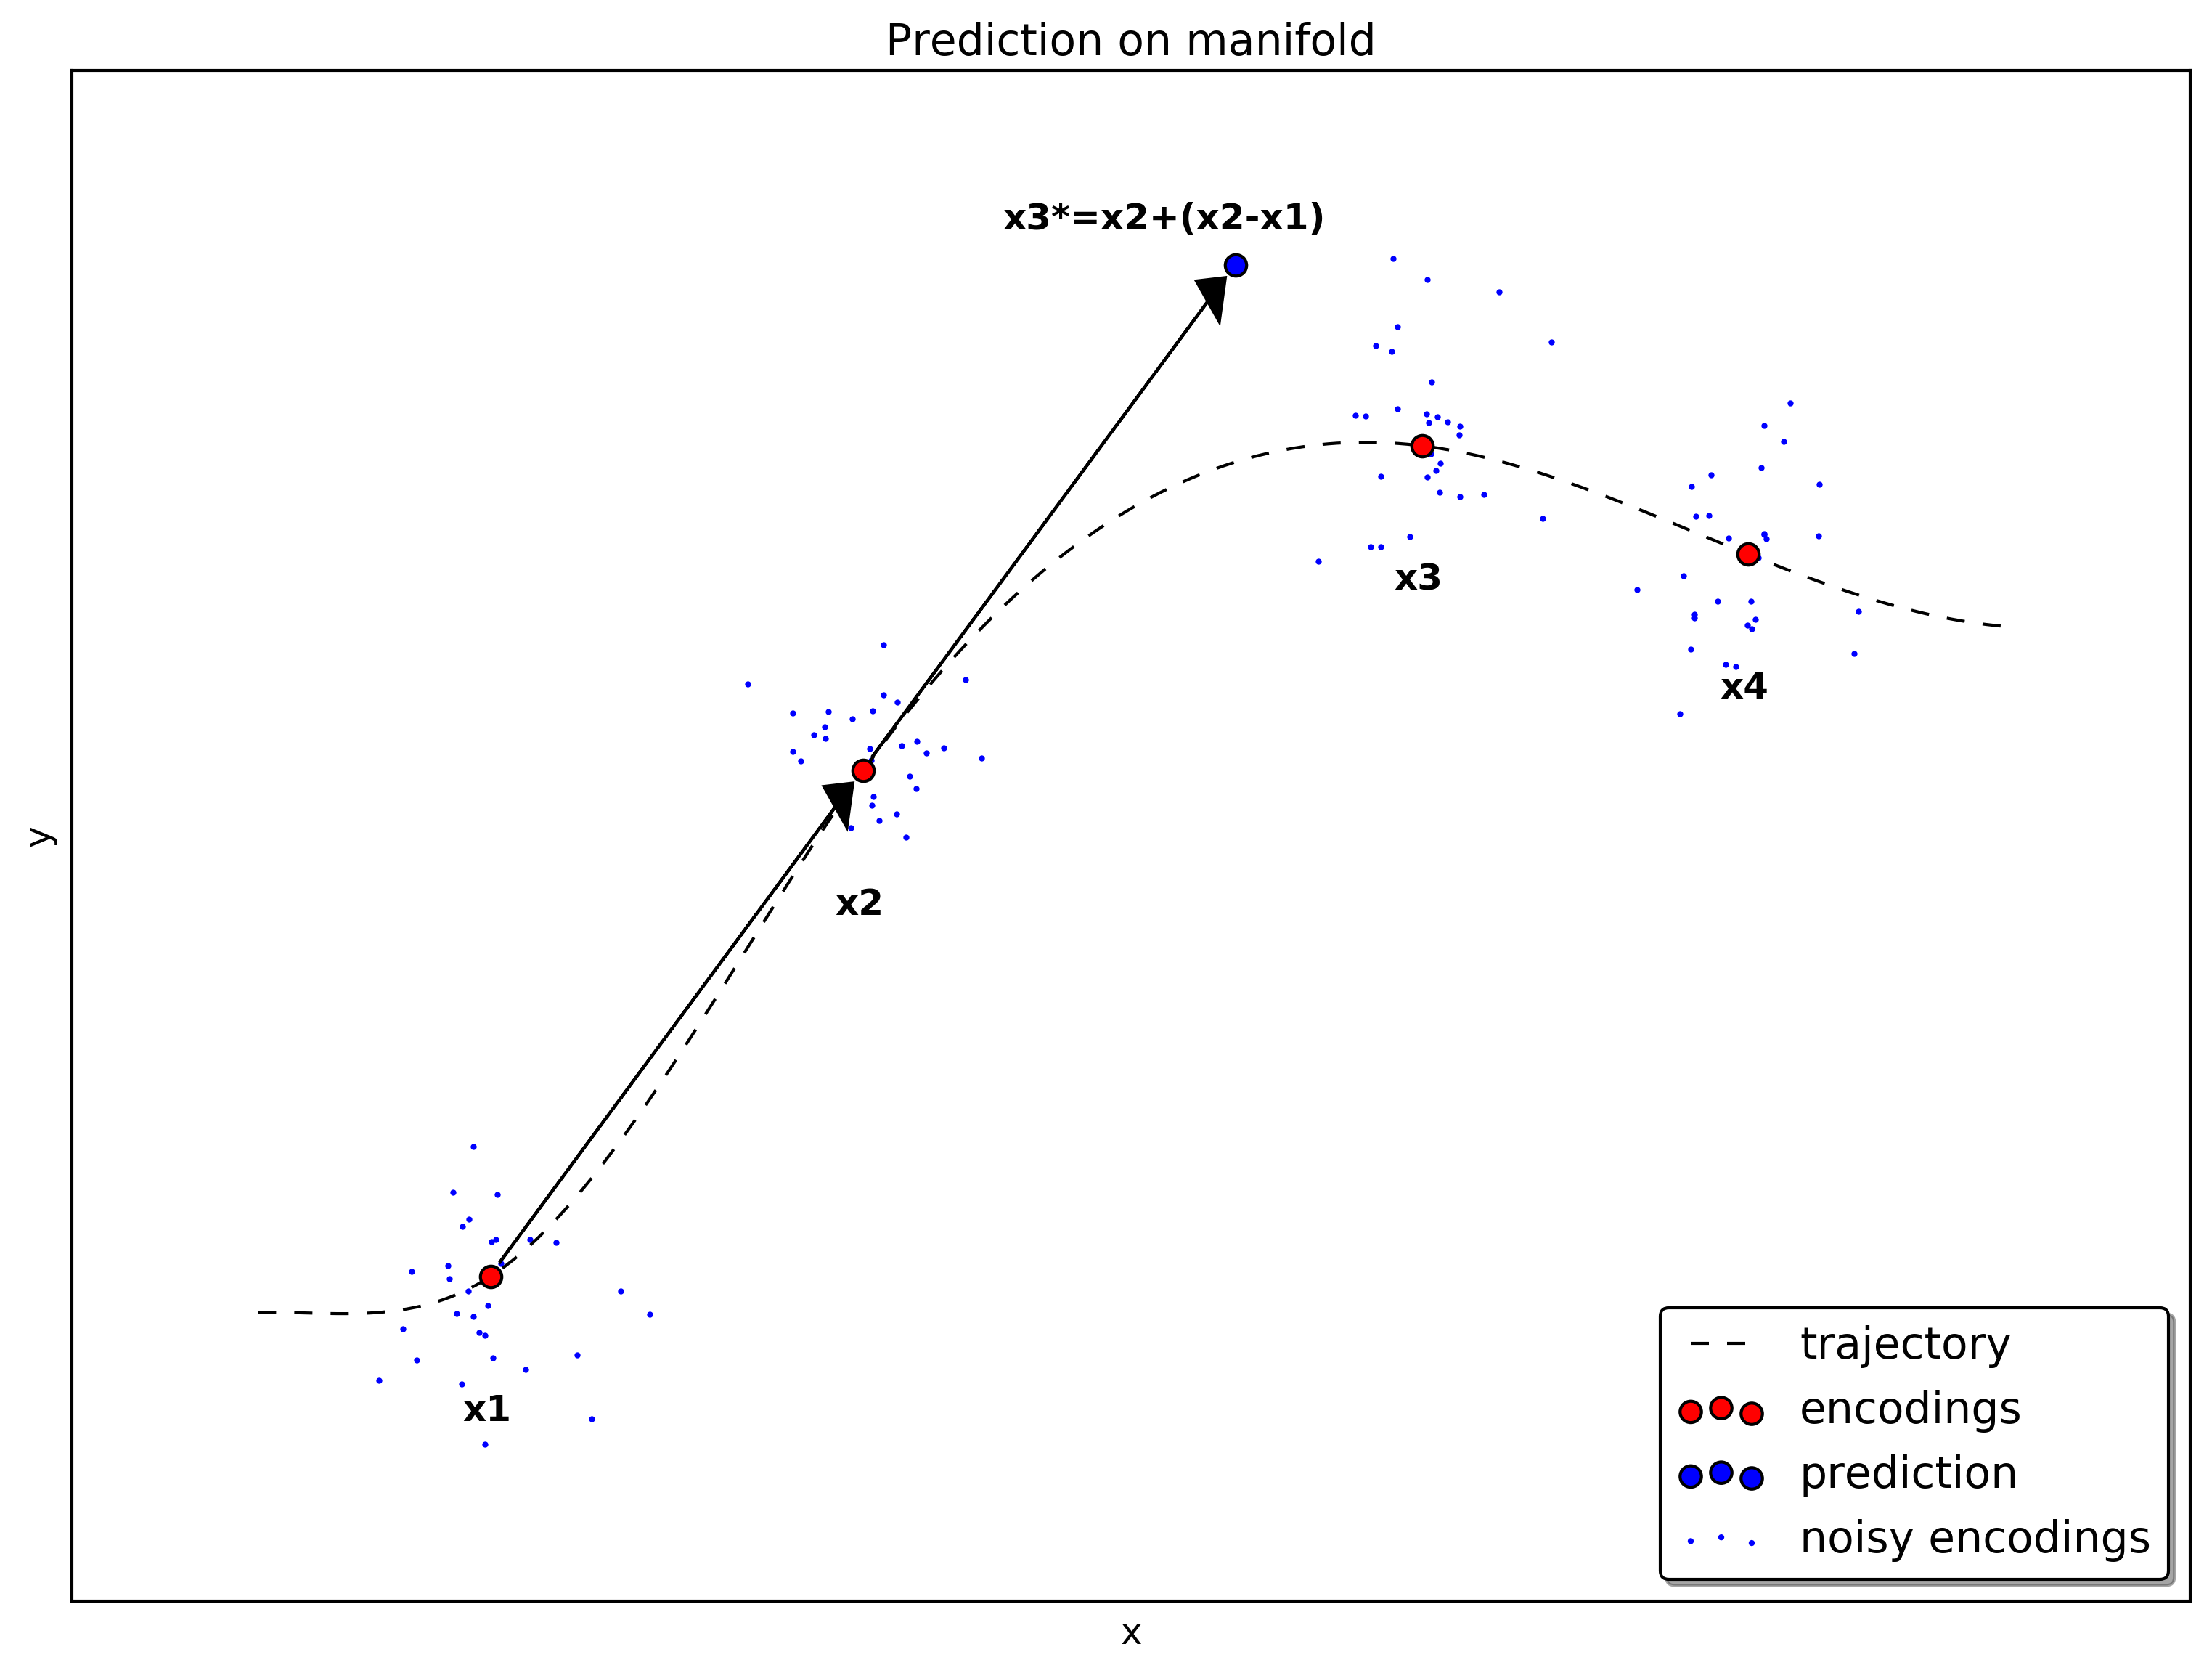
\includegraphics[width=0.75\textwidth,height=0.75\textheight,keepaspectratio]{images_main/prediction.png}
    \caption{Prediction on the spatial manifold.}
  \end{figure}
\end{frame}

% \begin{frame}{Regularization}
% \end{frame}

\begin{frame}{Model regularization}
  \begin{figure}
    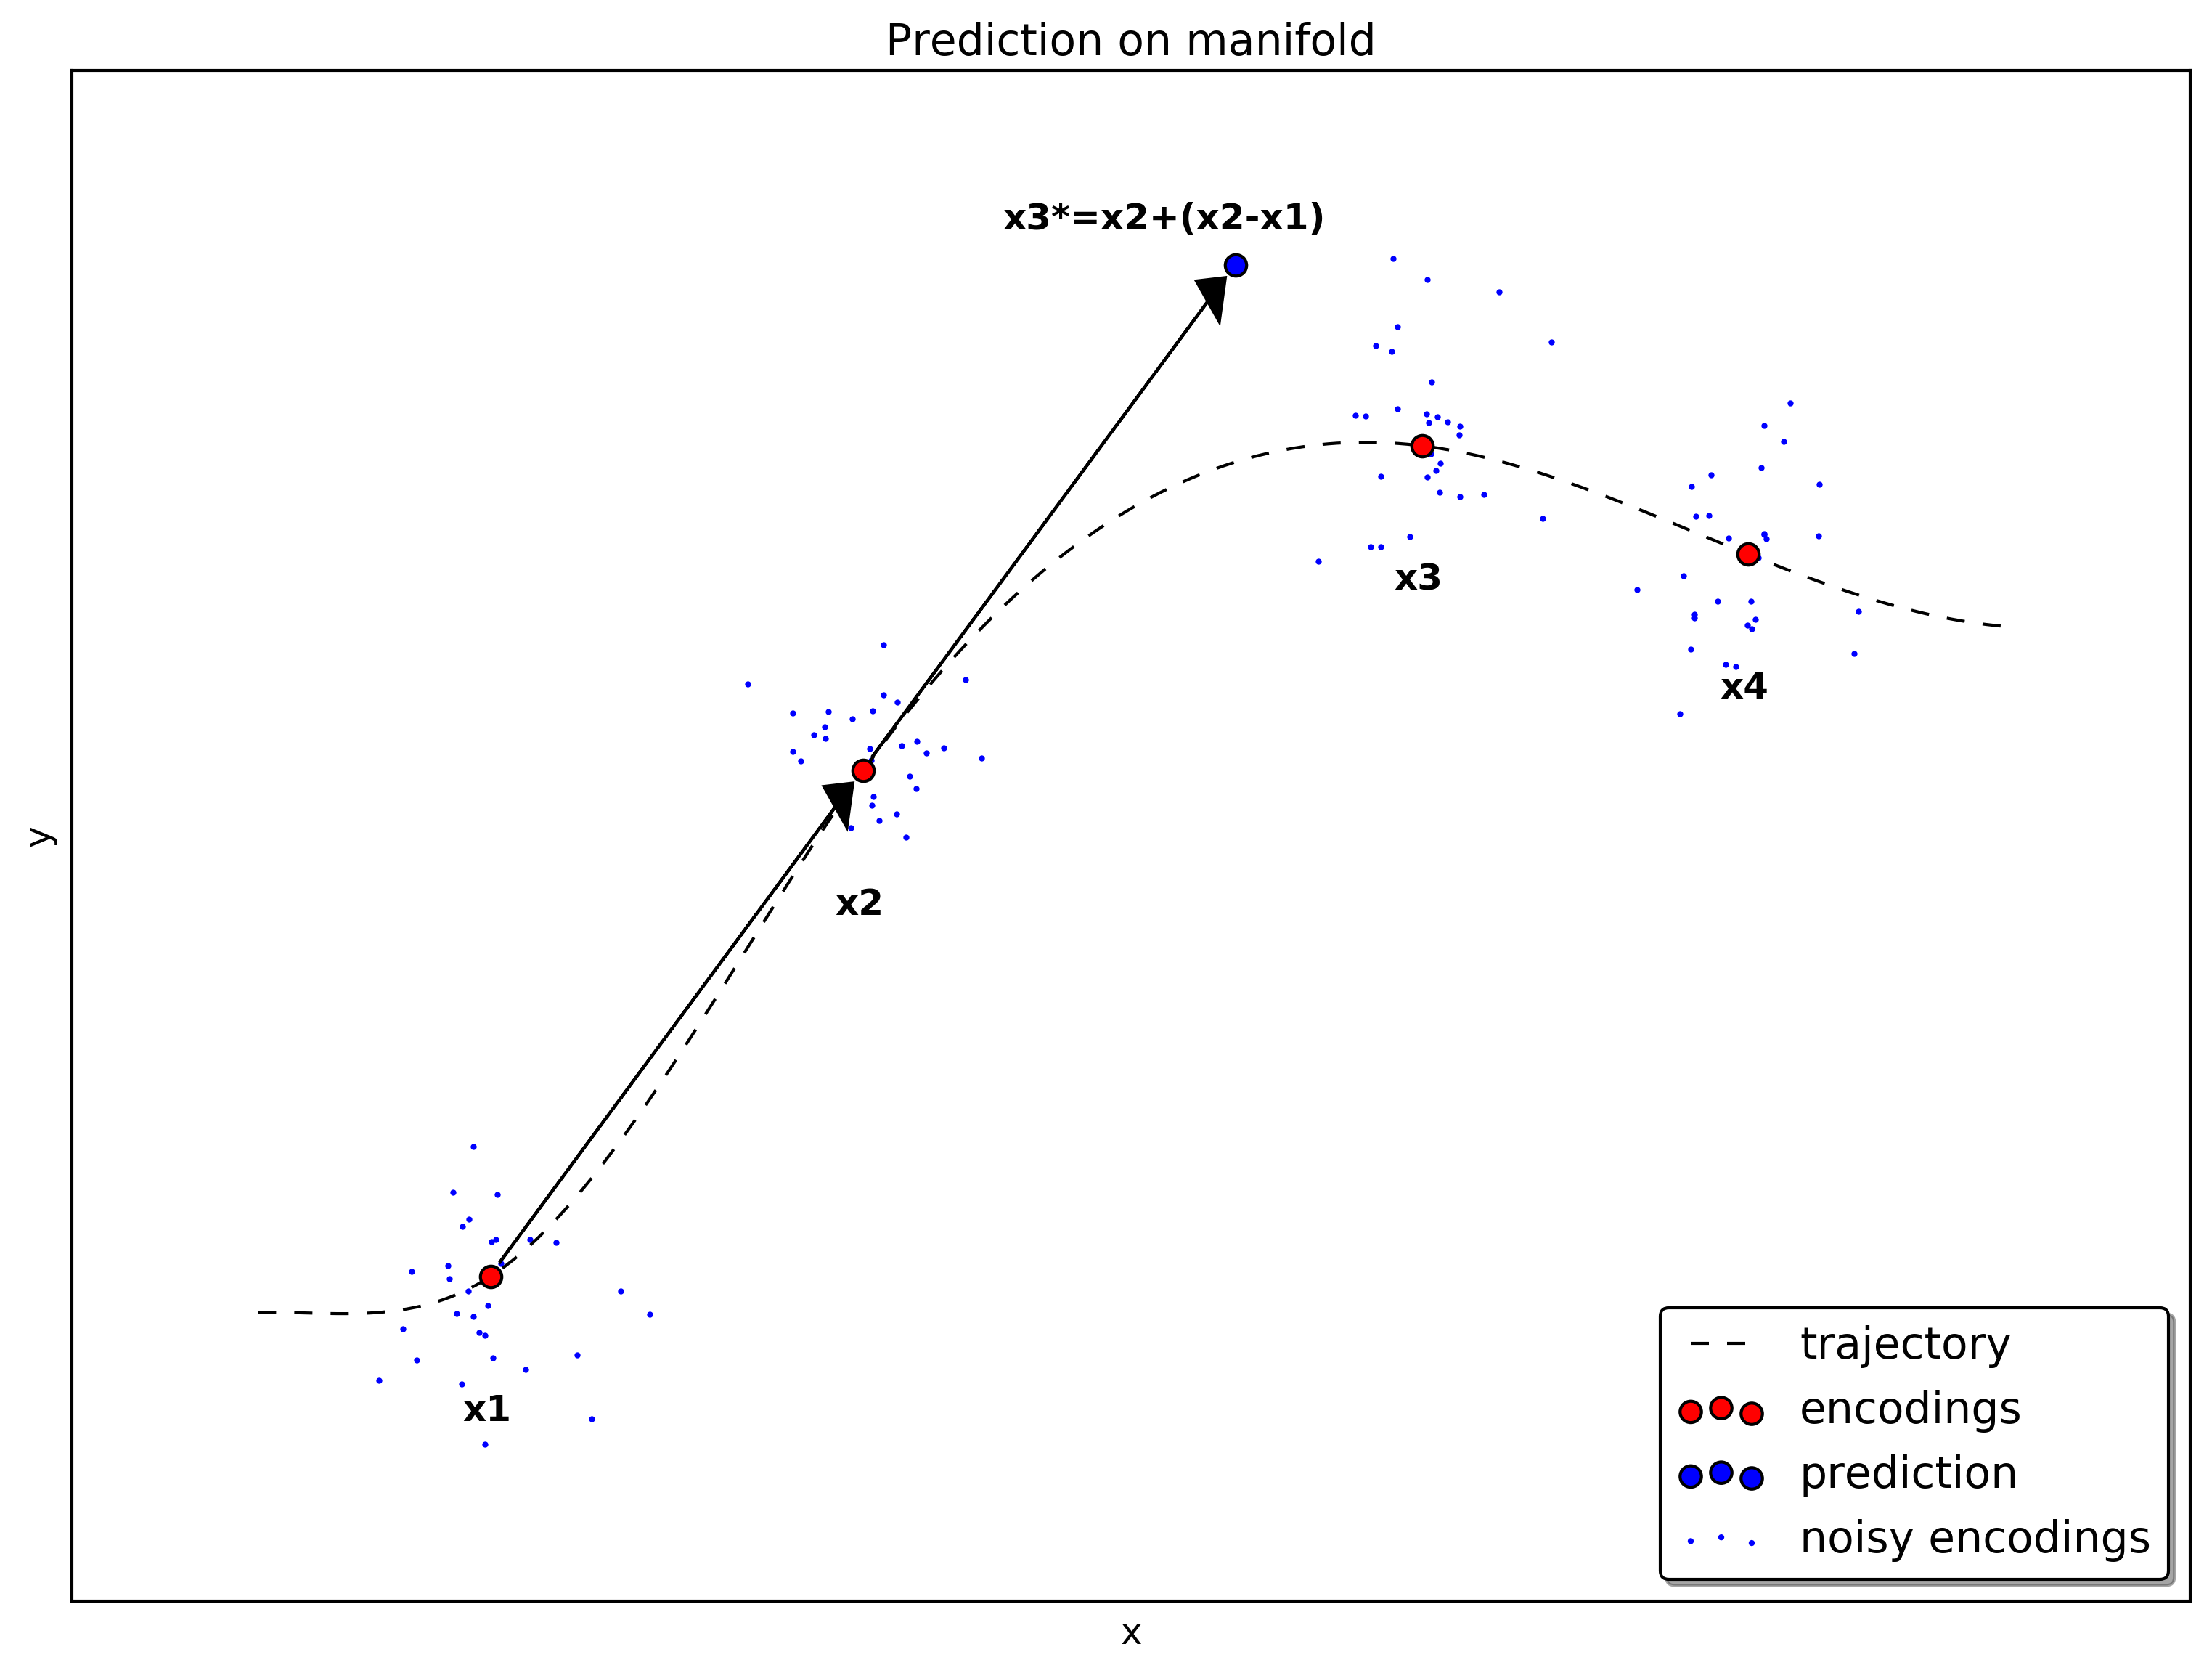
\includegraphics[width=0.75\textwidth,height=0.75\textheight,keepaspectratio]{images_main/prediction.png}
    \caption{Complete model with regularization.}
  \end{figure}
\end{frame}


\begin{frame}{Complete model structure}
  \begin{figure}
    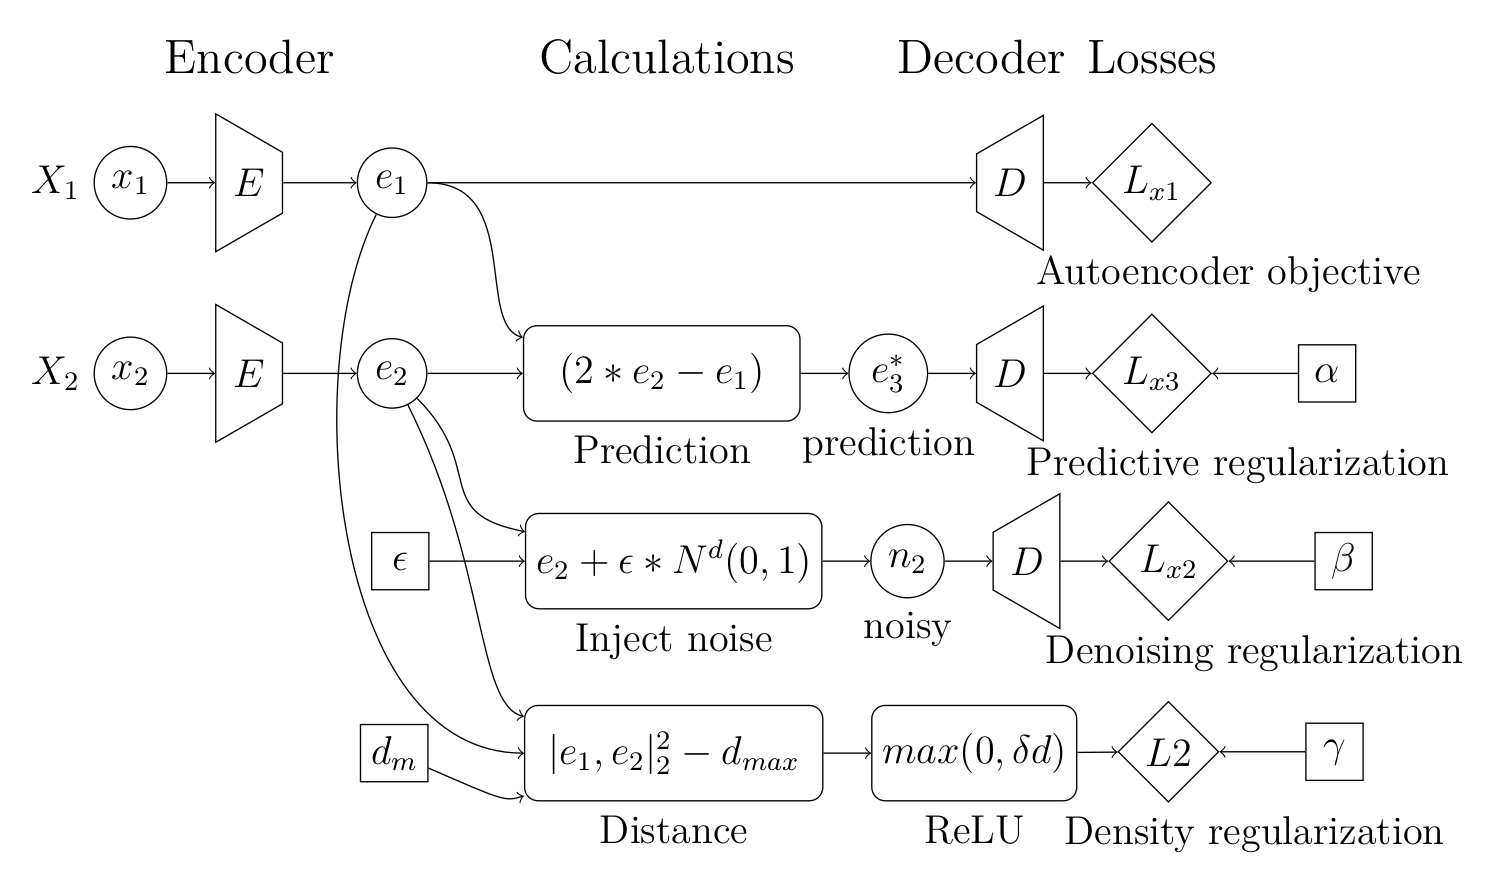
\includegraphics[width=0.9\textwidth,height=0.9\textheight,keepaspectratio]{images/model.png}
    \caption{Complete model with regularization.}
  \end{figure}
\end{frame}

\subsection{Metrics}

\begin{frame}
\end{frame}


\section{Evaluation}

\subsection{Data collection}

\begin{frame}
\end{frame}

\begin{frame}
\end{frame}


\subsection{Results}

\begin{frame}
\end{frame}

\begin{frame}
\end{frame}

\begin{frame}{Definition}
\end{frame}


\section*{Summary}

\begin{frame}
  \frametitle<presentation>{Summary}

  \begin{itemize}
  \item The \alert{first main message} of your talk in one or two lines.
  \end{itemize}

  % The following outlook is optional.
  \vskip0pt plus.5fill
  \begin{itemize}
  \item Outlook
    \begin{itemize}
    \item Something you haven't solved.
    \item Something else you haven't solved.
    \end{itemize}
  \end{itemize}
\end{frame}

\end{document}
